\section{Introducción}

\subsection{Antecedentes del programa espacial venezolano}

Particularmente llamativo resulta el esfuerzo de Venezuela por consolidar capacidades propias de observación terrestre a través del Sistema Venezolano de Satélites Remotos (VRSS). Lanzado en 2012, el VRSS-1 --conocido también como Francisco de Miranda-- marcó un hito al convertirse en el primer satélite de teledetección del país \cite{VRSS1_2012}. Operando en órbita heliosincrónica a aproximadamente 640 km de altitud, este satélite proporciona imágenes pancromáticas a 2.5 m y multiespectrales a 10 m, con capacidad para capturar hasta 350 imágenes diarias y múltiples pasadas sobre territorio nacional.

Aunque estas especificaciones espaciales resultan adecuadas para aplicaciones de cartografía, monitoreo de recursos naturales y apoyo en desastres, la arquitectura de un solo satélite impone restricciones inevitables. La revisita efectiva sobre áreas específicas tiende a oscilar entre varios días, limitando severamente su utilidad en escenarios dinámicos. 

\begin{table}[h]
\centering
\caption{Especificaciones principales de la plataforma VRSS-1 (adaptado de \cite{VRSS1_2012})}
\label{tab:especificaciones_vrss}
\begin{tabular}{ll}
\hline
\textbf{Parámetro} & \textbf{Valor} \\
\hline
Resolución pancromática & 2.5 m \\
Resolución multiespectral & 10 m \\
Altitud orbital & \sim 640 km \\
Tipo de órbita & Heliosincrónica \\
Revisita nominal & 4 días (global) \\
Imágenes diarias & \sim 350 \\
\hline
\end{tabular}
\end{table}

\subsection{Limitaciones de resolución temporal en EO}

Uno de los desafíos persistentes que surge al analizar sistemas de observación terrestre convencionales radica precisamente en el trade-off entre resolución espacial y temporal. Plataformas de alto rendimiento como VRSS entregan detalle geométrico excepcional, pero su capacidad para capturar procesos que evolucionan rápidamente --inundaciones repentinas, progresión de incendios, estrés hídrico en cultivos o movimientos de masas-- queda comprometida por intervalos de revisita que, en la práctica, suelen extenderse más allá de lo deseable.

Resulta revelador observar cómo la literatura reciente sobre observación de la Tierra con nanosatélites ha transformado esta ecuación \cite{Nagel2020}. Constelaciones de CubeSats demuestran que es posible lograr coberturas temporales de horas o incluso minutos sin sacrificar enteramente la calidad radiométrica. Lejos de ser una solución marginal, esta aproximación ha pasado de experimentos académicos a operaciones comerciales maduras, revelando limitaciones estructurales de los sistemas basados en plataformas individuales de gran tamaño.

\subsection{Contribuciones del trabajo}

En este contexto, el presente trabajo propone la integración de una red de nanosatélites como sistema complementario a la infraestructura VRSS existente. Lejos de reemplazar la plataforma principal, la arquitectura híbrida busca potenciar sus fortalezas espaciales con la agilidad temporal inherente a las constelaciones distribuidas.

Las contribuciones principales incluyen: (i) el diseño de una topología orbital optimizada que maximice la complementariedad con las órbitas VRSS; (ii) un marco de fusión de datos multi-sensor que preserve la alta resolución espacial mientras eleva drásticamente la frecuencia de actualización; y (iii) una evaluación cuantitativa de las mejoras en continuidad y resolución temporal mediante simulaciones realistas. 

Aplicaciones de constelaciones de nanosatélites en monitoreo ambiental y detección temprana, tal como se documenta ampliamente \cite{Kerrouche2023}, respaldan la viabilidad técnica de esta integración. De esta manera, se aspira a ofrecer una solución costo-efectiva y escalable que fortalezca las capacidades nacionales de observación terrestre en un escenario de crecientes demandas por datos oportunos.

\begin{figure}[h]
\centering
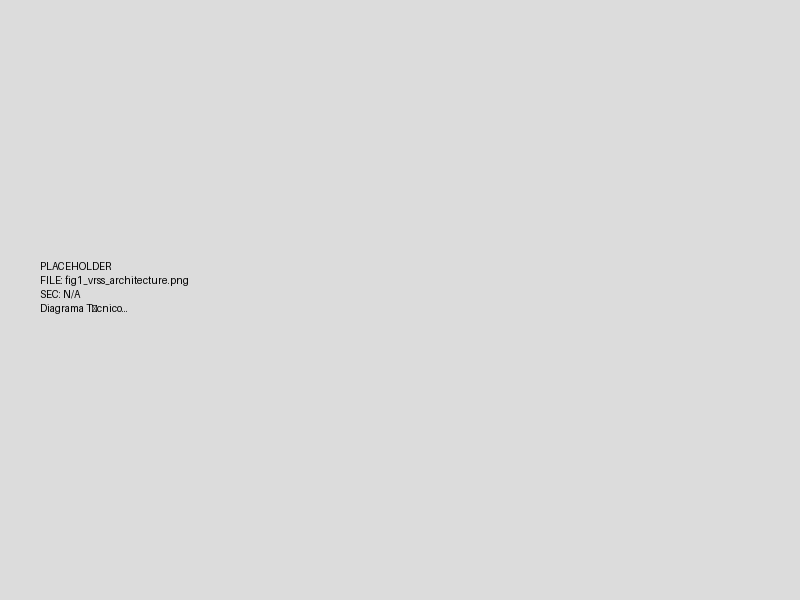
\includegraphics[width=\linewidth]{fig1_vrss_architecture.png}
\caption{Arquitectura general del sistema VRSS y su integración conceptual con la red de nanosatélites propuesta.}
\label{fig:arquitectura_vrss}
\end{figure}